% !TEX encoding = UTF-8 Unicode

%% bare_jrnl.tex
%% V1.4
%% 2012/12/27
%% by Michael Shell
%% see http://www.michaelshell.org/
%% for current contact information.
%%
%% This is a skeleton file demonstrating the use of IEEEtran.cls
%% (requires IEEEtran.cls version 1.8 or later) with an IEEE journal paper.
%%
%% Support sites:
%% http://www.michaelshell.org/tex/ieeetran/
%% http://www.ctan.org/tex-archive/macros/latex/contrib/IEEEtran/
%% and
%% http://www.ieee.org/



% *** Authors should verify (and, if needed, correct) their LaTeX system  ***
% *** with the testflow diagnostic prior to trusting their LaTeX platform ***
% *** with production work. IEEE's font choices can trigger bugs that do  ***
% *** not appear when using other class files.&***
% The testflow support page is at:
% http://www.michaelshell.org/tex/testflow/


%%*************************************************************************
%% Legal Notice:
%% This code is offered as-is without any warranty either expressed or
%% implied; without even the implied warranty of MERCHANTABILITY or
%% FITNESS FOR A PARTICULAR PURPOSE! 
%% User assumes all risk.
%% In no event shall IEEE or any contributor to this code be liable for
%% any damages or losses, including, but not limited to, incidental,
%% consequential, or any other damages, resulting from the use or misuse
%% of any information contained here.
%%
%% All comments are the opinions of their respective authors and are not
%% necessarily endorsed by the IEEE.
%%
%% This work is distributed under the LaTeX Project Public License (LPPL)
%% ( http://www.latex-project.org/ ) version 1.3, and may be freely used,
%% distributed and modified. A copy of the LPPL, version 1.3, is included
%% in the base LaTeX documentation of all distributions of LaTeX released
%% 2003/12/01 or later.
%% Retain all contribution notices and credits.
%% ** Modified files should be clearly indicated as such, including  **
%% ** renaming them and changing author support contact information. **
%%
%% File list of work: IEEEtran.cls, IEEEtran_HOWTO.pdf, bare_adv.tex,
%%& bare_conf.tex, bare_jrnl.tex, bare_jrnl_compsoc.tex,
%%& bare_jrnl_transmag.tex
%%*************************************************************************

% Note that the a4paper option is mainly intended so that authors in
% countries using A4 can easily print to A4 and see how their papers will
% look in print - the typesetting of the document will not typically be
% affected with changes in paper size (but the bottom and side margins will).
% Use the testflow package mentioned above to verify correct handling of
% both paper sizes by the user's LaTeX system.
%
% Also note that the "draftcls" or "draftclsnofoot", not "draft", option
% should be used if it is desired that the figures are to be displayed in
% draft mode.
%
\documentclass[journal]{IEEEtran}
%
% If IEEEtran.cls has not been installed into the LaTeX system files,
% manually specify the path to it like:
% \documentclass[journal]{../sty/IEEEtran}





% Some very useful LaTeX packages include:
% (uncomment the ones you want to load)


% *** MISC UTILITY PACKAGES ***
\usepackage{verbatim}
\usepackage[font=small]{caption}
\usepackage[utf8]{inputenc}
\usepackage{amssymb}
\usepackage[table]{xcolor}
%\usepackage[autolinebreaks,framed]{mcode} %matlab code
%\lstset{breakatwhitespace=false}
%
%\usepackage{ifpdf}
% Heiko Oberdiek's ifpdf.sty is very useful if you need conditional
% compilation based on whether the output is pdf or dvi.
% usage:
% \ifpdf
%   % pdf code
% \else
%   % dvi code
% \fi
% The latest version of ifpdf.sty can be obtained from:
% http://www.ctan.org/tex-archive/macros/latex/contrib/oberdiek/
% Also, note that IEEEtran.cls V1.7 and later provides a builtin
% \ifCLASSINFOpdf conditional that works the same way.
% When switching from latex to pdflatex and vice-versa, the compiler may
% have to be run twice to clear warning/error messages.






% *** CITATION PACKAGES ***
%
%\usepackage{cite}
% cite.sty was written by Donald Arseneau
% V1.6 and later of IEEEtran pre-defines the format of the cite.sty package
% \cite{} output to follow that of IEEE. Loading the cite package will
% result in citation numbers being automatically sorted and properly
% "compressed/ranged". e.g., [1], [9], [2], [7], [5], [6] without using
% cite.sty will become [1], [2], [5]--[7], [9] using cite.sty. cite.sty's
% \cite will automatically add leading space, if needed. Use cite.sty's
% noadjust option (cite.sty V3.8 and later) if you want to turn this off
% such as if a citation ever needs to be enclosed in parenthesis.
% cite.sty is already installed on most LaTeX systems. Be sure and use
% version 4.0 (2003-05-27) and later if using hyperref.sty. cite.sty does
% not currently provide for hyperlinked citations.
% The latest version can be obtained at:
% http://www.ctan.org/tex-archive/macros/latex/contrib/cite/
% The documentation is contained in the cite.sty file itself.






% *** GRAPHICS RELATED PACKAGES ***
%
\ifCLASSINFOpdf
\usepackage[pdftex]{graphicx}
  % declare the path(s) where your graphic files are
  \graphicspath{}
  % and their extensions so you won't have to specify these with
  % every instance of \includegraphics
\DeclareGraphicsExtensions{.png}
\else
  % or other class option (dvipsone, dvipdf, if not using dvips). graphicx
  % will default to the driver specified in the system graphics.cfg if no
  % driver is specified.
  % \usepackage[dvips]{graphicx}
  % declare the path(s) where your graphic files are
  % \graphicspath{{../eps/}}
  % and their extensions so you won't have to specify these with
  % every instance of \includegraphics
  % \DeclareGraphicsExtensions{.eps}
\fi
% graphicx was written by David Carlisle and Sebastian Rahtz. It is
% required if you want graphics, photos, etc. graphicx.sty is already
% installed on most LaTeX systems. The latest version and documentation
% can be obtained at: 
% http://www.ctan.org/tex-archive/macros/latex/required/graphics/
% Another good source of documentation is "Using Imported Graphics in
% LaTeX2e" by Keith Reckdahl which can be found at:
% http://www.ctan.org/tex-archive/info/epslatex/
%
% latex, and pdflatex in dvi mode, support graphics in encapsulated
% postscript (.eps) format. pdflatex in pdf mode supports graphics
% in .pdf, .jpeg, .png and .mps (metapost) formats. Users should ensure
% that all non-photo figures use a vector format (.eps, .pdf, .mps) and
% not a bitmapped formats (.jpeg, .png). IEEE frowns on bitmapped formats
% which can result in "jaggedy"/blurry rendering of lines and letters as
% well as large increases in file sizes.
%
% You can find documentation about the pdfTeX application at:
% http://www.tug.org/applications/pdftex





% *** MATH PACKAGES ***
%
\usepackage[cmex10]{amsmath}
% A popular package from the American Mathematical Society that provides
% many useful and powerful commands for dealing with mathematics. If using
% it, be sure to load this package with the cmex10 option to ensure that
% only type 1 fonts will utilized at all point sizes. Without this option,
% it is possible that some math symbols, particularly those within
% footnotes, will be rendered in bitmap form which will result in a
% document that can not be IEEE Xplore compliant!
%
% Also, note that the amsmath package sets \interdisplaylinepenalty to 10000
% thus preventing page breaks from occurring within multiline equations. Use:
%\interdisplaylinepenalty=2500
% after loading amsmath to restore such page breaks as IEEEtran.cls normally
% does. amsmath.sty is already installed on most LaTeX systems. The latest
% version and documentation can be obtained at:
% http://www.ctan.org/tex-archive/macros/latex/required/amslatex/math/





% *** SPECIALIZED LIST PACKAGES ***
%
%\usepackage{algorithmic}
% algorithmic.sty was written by Peter Williams and Rogerio Brito.
% This package provides an algorithmic environment fo describing algorithms.
% You can use the algorithmic environment in-text or within a figure
% environment to provide for a floating algorithm. Do NOT use the algorithm
% floating environment provided by algorithm.sty (by the same authors) or
% algorithm2e.sty (by Christophe Fiorio) as IEEE does not use dedicated
% algorithm float types and packages that provide these will not provide
% correct IEEE style captions. The latest version and documentation of
% algorithmic.sty can be obtained at:
% http://www.ctan.org/tex-archive/macros/latex/contrib/algorithms/
% There is also a support site at:
% http://algorithms.berlios.de/index.html
% Also of interest may be the (relatively newer and more customizable)
% algorithmicx.sty package by Szasz Janos:
% http://www.ctan.org/tex-archive/macros/latex/contrib/algorithmicx/




% *** ALIGNMENT PACKAGES ***
%
\usepackage{array}
% Frank Mittelbach's and David Carlisle's array.sty patches and improves
% the standard LaTeX2e array and tabular environments to provide better
% appearance and additional user controls. As the default LaTeX2e table
% generation code is lacking to the point of almost being broken with
% respect to the quality of the end results, all users are strongly
% advised to use an enhanced (at the very least that provided by array.sty)
% set of table tools. array.sty is already installed on most systems. The
% latest version and documentation can be obtained at:
% http://www.ctan.org/tex-archive/macros/latex/required/tools/


% IEEEtran contains the IEEEeqnarray family of commands that can be used to
% generate multiline equations as well as matrices, tables, etc., of high
% quality.




% *** SUBFIGURE PACKAGES ***
%\ifCLASSOPTIONcompsoc
%  \usepackage[caption=false,font=normalsize,labelfont=sf,textfont=sf]{subfig}
%\else
%  \usepackage[caption=false,font=footnotesize]{subfig}
%\fi
% subfig.sty, written by Steven Douglas Cochran, is the modern replacement
% for subfigure.sty, the latter of which is no longer maintained and is
% incompatible with some LaTeX packages including fixltx2e. However,
% subfig.sty requires and automatically loads Axel Sommerfeldt's caption.sty
% which will override IEEEtran.cls' handling of captions and this will result
% in non-IEEE style figure/table captions. To prevent this problem, be sure
% and invoke subfig.sty's "caption=false" package option (available since
% subfig.sty version 1.3, 2005/06/28) as this is will preserve IEEEtran.cls
% handling of captions.
% Note that the Computer Society format requires a larger sans serif font
% than the serif footnote size font used in traditional IEEE formatting
% and thus the need to invoke different subfig.sty package options depending
% on whether compsoc mode has been enabled.
%
% The latest version and documentation of subfig.sty can be obtained at:
% http://www.ctan.org/tex-archive/macros/latex/contrib/subfig/




% *** FLOAT PACKAGES ***
%
%\usepackage{fixltx2e}
% fixltx2e, the successor to the earlier fix2col.sty, was written by
% Frank Mittelbach and David Carlisle. This package corrects a few problems
% in the LaTeX2e kernel, the most notable of which is that in current
% LaTeX2e releases, the ordering of single and double column floats is not
% guaranteed to be preserved. Thus, an unpatched LaTeX2e can allow a
% single column figure to be placed prior to an earlier double column
% figure. The latest version and documentation can be found at:
% http://www.ctan.org/tex-archive/macros/latex/base/


%\usepackage{stfloats}
% stfloats.sty was written by Sigitas Tolusis. This package gives LaTeX2e
% the ability to do double column floats at the bottom of the page as well
% as the top. (e.g., "\begin{figure*}[!b]" is not normally possible in
% LaTeX2e). It also provides a command:
%\fnbelowfloat
% to enable the placement of footnotes below bottom floats (the standard
% LaTeX2e kernel puts them above bottom floats). This is an invasive package
% which rewrites many portions of the LaTeX2e float routines. It may not work
% with other packages that modify the LaTeX2e float routines. The latest
% version and documentation can be obtained at:
% http://www.ctan.org/tex-archive/macros/latex/contrib/sttools/
% Do not use the stfloats baselinefloat ability as IEEE does not allow
% \baselineskip to stretch. Authors submitting work to the IEEE should note
% that IEEE rarely uses double column equations and that authors should try
% to avoid such use. Do not be tempted to use the cuted.sty or midfloat.sty
% packages (also by Sigitas Tolusis) as IEEE does not format its papers in
% such ways.
% Do not attempt to use stfloats with fixltx2e as they are incompatible.
% Instead, use Morten Hogholm'a dblfloatfix which combines the features
% of both fixltx2e and stfloats:
%
% \usepackage{dblfloatfix}
% The latest version can be found at:
% http://www.ctan.org/tex-archive/macros/latex/contrib/dblfloatfix/




%\ifCLASSOPTIONcaptionsoff
%  \usepackage[nomarkers]{endfloat}
% \let\MYoriglatexcaption\caption
% \renewcommand{\caption}[2][\relax]{\MYoriglatexcaption[#2]{#2}}
%\fi
% endfloat.sty was written by James Darrell McCauley, Jeff Goldberg and 
% Axel Sommerfeldt. This package may be useful when used in conjunction with 
% IEEEtran.cls'  captionsoff option. Some IEEE journals/societies require that
% submissions have lists of figures/tables at the end of the paper and that
% figures/tables without any captions are placed on a page by themselves at
% the end of the document. If needed, the draftcls IEEEtran class option or
% \CLASSINPUTbaselinestretch interface can be used to increase the line
% spacing as well. Be sure and use the nomarkers option of endfloat to
% prevent endfloat from "marking" where the figures would have been placed
% in the text. The two hack lines of code above are a slight modification of
% that suggested by in the endfloat docs (section 8.4.1) to ensure that
% the full captions always appear in the list of figures/tables - even if
% the user used the short optional argument of \caption[]{}.
% IEEE papers do not typically make use of \caption[]'s optional argument,
% so this should not be an issue. A similar trick can be used to disable
% captions of packages such as subfig.sty that lack options to turn off
% the subcaptions:
% For subfig.sty:
% \let\MYorigsubfloat\subfloat
% \renewcommand{\subfloat}[2][\relax]{\MYorigsubfloat[]{#2}}
% However, the above trick will not work if both optional arguments of
% the \subfloat command are used. Furthermore, there needs to be a
% description of each subfigure *somewhere* and endfloat does not add
% subfigure captions to its list of figures. Thus, the best approach is to
% avoid the use of subfigure captions (many IEEE journals avoid them anyway)
% and instead reference/explain all the subfigures within the main caption.
% The latest version of endfloat.sty and its documentation can obtained at:
% http://www.ctan.org/tex-archive/macros/latex/contrib/endfloat/
%
% The IEEEtran \ifCLASSOPTIONcaptionsoff conditional can also be used
% later in the document, say, to conditionally put the References on a 
% page by themselves.




% *** PDF, URL AND HYPERLINK PACKAGES ***
%
%\usepackage{url}
% url.sty was written by Donald Arseneau. It provides better support for
% handling and breaking URLs. url.sty is already installed on most LaTeX
% systems. The latest version and documentation can be obtained at:
% http://www.ctan.org/tex-archive/macros/latex/contrib/url/
% Basically, \url{my_url_here}.




% *** Do not adjust lengths that control margins, column widths, etc. ***
% *** Do not use packages that alter fonts (such as pslatex).&***
% There should be no need to do such things with IEEEtran.cls V1.6 and later.
% (Unless specifically asked to do so by the journal or conference you plan
% to submit to, of course. )


% correct bad hyphenation here
\hyphenation{op-tical net-works semi-conduc-tor}
 
\begin{document}
%
% paper title
% can use linebreaks \\ within to get better formatting as desired
% Do not put math or special symbols in the title.
\title{Plataformas de Servicio en Redes M2M y Modelamiento de algunas Aplicaciones}
%
%
% author names and IEEE memberships
% note positions of commas and nonbreaking spaces ( ~ ) LaTeX will not break
% a structure at a ~ so this keeps an author's name from being broken across
% two lines.
% use \thanks{} to gain access to the first footnote area
% a separate \thanks must be used for each paragraph as LaTeX2e's \thanks
% was not built to handle multiple paragraphs
%

\author{Juan Sebastian Martinez, 201125846. Andrés Alba, 201124622}% <-this % stops a space
% note the % following the last \IEEEmembership and also \thanks - 
% these prevent an unwanted space from occurring between the last author name
% and the end of the author line. i.e., if you had this:
% 
% \author{....lastname \thanks{...} \thanks{...} }
%&  ^------------^------------^----Do not want these spaces!
%
% a space would be appended to the last name and could cause every name on that
% line to be shifted left slightly. This is one of those "LaTeX things". For
% instance, "\textbf{A} \textbf{B}" will typeset as "A B" not "AB". To get
% "AB" then you have to do: "\textbf{A}\textbf{B}"
% \thanks is no different in this regard, so shield the last } of each \thanks
% that ends a line with a % and do not let a space in before the next \thanks.
% Spaces after \IEEEmembership other than the last one are OK (and needed) as
% you are supposed to have spaces between the names. For what it is worth,
% this is a minor point as most people would not even notice if the said evil
% space somehow managed to creep in.



% The paper headers
\markboth{Universidad de los Andes - Ingeniería de Teletráfico}%
{}
% The only time the second header will appear is for the odd numbered pages
% after the title page when using the twoside option.
% 
% *** Note that you probably will NOT want to include the author's ***
% *** name in the headers of peer review papers.&***
% You can use \ifCLASSOPTIONpeerreview for conditional compilation here if
% you desire.




% If you want to put a publisher's ID mark on the page you can do it like
% this:
%\IEEEpubid{0000--0000/00\$00.00~\copyright~2012 IEEE}
% Remember, if you use this you must call \IEEEpubidadjcol in the second
% column for its text to clear the IEEEpubid mark.



% use for special paper notices
%\IEEEspecialpapernotice{(Invited Paper)}




% make the title area
\maketitle

% As a general rule, do not put math, special symbols or citations
% in the abstract or keywords.
\begin{abstract}
Las redes Machine-to-Machine (M2M) son un área de gran interes en la actualidad debido a sus amplias aplicaciones. Gracias a esto, es pertinente  el estudio de este tipo de redes bajo un criterio de estandarización, donde se presenten los requisitos ideales de una plataforma de servicio M2M (M2SP) y su respectiva arquitectura.\\
En el siguiente documento, se realiza un estudio de actualidad de las redes M2M para presentar dicha plataforma ideal de servicio; a su vez, para ilustrar las características de la plataforma, se presentan dos casos especificos de estas redes, como lo son las redes de dispositivos móviles y el modelo markoviano de sistemas de recepción discontinua (DRX); y los modelos basados en procesos de markov modulados (CMMPP) para las fuentes de tráfico de redes M2M.
\end{abstract}

% Note that keywords are not normally used for peerreview papers.
\begin{IEEEkeywords}
Arquitectura, Coupled Markov Modulation Poisson Process, Discontinuous Reception, Machine-to-Machine, Plataforma de Servicio.
\end{IEEEkeywords}






% For peer review papers, you can put extra information on the cover
% page as needed:
% \ifCLASSOPTIONpeerreview
% \begin{center} \bfseries EDICS Category: 3-BBND \end{center}
% \fi
%
% For peerreview papers, this IEEEtran command inserts a page break and
% creates the second title. It will be ignored for other modes.
\IEEEpeerreviewmaketitle



\section{Introducci\'on}
% The very first letter is a 2 line initial drop letter followed
% by the rest of the first word in caps.
% 
% form to use if the first word consists of a single letter:
% \IEEEPARstart{A}{demo} file is ....
% 
% form to use if you need the single drop letter followed by
% normal text (unknown if ever used by IEEE):
% \IEEEPARstart{A}{}demo file is ....
% 
% Some journals put the first two words in caps:
% \IEEEPARstart{T}{his demo} file is ....
% 
% Here we have the typical use of a "T" for an initial drop letter
% and "HIS" in caps to complete the first word.
\IEEEPARstart{L}{a}s redes Machine-to-Machine definen redes de comunicación entre máquinas donde la intervención humana es nula. Estas redes estan compuestas por varios tipos de máquinas y pueden ser redes alámbricas o inalámbricas. Gracias a los diversos tipos de dispositivos y objetivos de estas redes, existen en la actualidad una gran variedad de arquitecturas y protocolos para estas redes dependiendo de su aplicación.\\

Dentro de dichas aplicaciones se encuentran las redes de sensores, redes de seguridad pública y protección civil, Smart Grids, sistemas de transporte inteligente (ITS), aplicaciones militares, etc.\\

Gracias a esta gran diversidad, resulta intersante la realización de un estudio sobre la naturaleza de las comunicaciones M2M con el fin de describir sus principales características y requerimientos. Bajo estos criterios, es posible definir una plataforma de servicio general, que pueda servir a los requisitos de las redes bajo una arquitectura definida.\\

A continuación se presenta un estudio sobre las redes M2M que permite definir los criterios anteriores; se realiza una descripción de las principales características de las redes, las plataformas existentes y la proposición de una plataforma de servicio M2SP junto con una recopilación de tecnologías y estándares que la plataforma debe cumplir.\\

Por último, se ilustran dos casos de estudio de este tipo de redes en donde el modelamiento del tráfico y los modelos de probabilidad son importantes para el entendimiento de la red.
 
% You must have at least 2 lines in the paragraph with the drop letter
% (should never be an issue)


%\subsection{Subsection Heading Here}
%Subsection text here.

% needed in second column of first page if using \IEEEpubid
%\IEEEpubidadjcol

%\subsubsection{Subsubsection Heading Here}
%Subsubsection text here.


% An example of a floating figure using the graphicx package.
% Note that \label must occur AFTER (or within) \caption.
% For figures, \caption should occur after the \includegraphics.
% Note that IEEEtran v1.7 and later has special internal code that
% is designed to preserve the operation of \label within \caption
% even when the captionsoff option is in effect. However, because
% of issues like this, it may be the safest practice to put all your
% \label just after \caption rather than within \caption{}.
%
% Reminder: the "draftcls" or "draftclsnofoot", not "draft", class
% option should be used if it is desired that the figures are to be
% displayed while in draft mode.
%
%\begin{figure}[!t]
%\centering
%\includegraphics[width=2.5in]{myfigure}
% where an .eps filename suffix will be assumed under latex, 
% and a .pdf suffix will be assumed for pdflatex; or what has been declared
% via \DeclareGraphicsExtensions.
%\caption{Simulation Results.}
%\label{fig_sim}
%\end{figure}

% Note that IEEE typically puts floats only at the top, even when this
% results in a large percentage of a column being occupied by floats.


% An example of a double column floating figure using two subfigures.
% (The subfig.sty package must be loaded for this to work.)
% The subfigure \label commands are set within each subfloat command,
% and the \label for the overall figure must come after \caption.
% \hfil is used as a separator to get equal spacing.
% Watch out that the combined width of all the subfigures on a 
% line do not exceed the text width or a line break will occur.
%
%\begin{figure*}[!t]
%\centering
%\subfloat[Case I]{\includegraphics[width=2.5in]{box}%
%\label{fig_first_case}}
%\hfil
%\subfloat[Case II]{\includegraphics[width=2.5in]{box}%
%\label{fig_second_case}}
%\caption{Simulation results.}
%\label{fig_sim}
%\end{figure*}
%
% Note that often IEEE papers with subfigures do not employ subfigure
% captions (using the optional argument to \subfloat[]), but instead will
% reference/describe all of them (a), (b), etc., within the main caption.


% An example of a floating table. Note that, for IEEE style tables, the 
% \caption command should come BEFORE the table. Table text will default to
% \footnotesize as IEEE normally uses this smaller font for tables.
% The \label must come after \caption as always.
%
%\begin{table}[!t]
%% increase table row spacing, adjust to taste
%\renewcommand{\arraystretch}{1.3}
% if using array.sty, it might be a good idea to tweak the value of
% \extrarowheight as needed to properly center the text within the cells
%\caption{An Example of a Table}
%\label{table_example}
%\centering
%% Some packages, such as MDW tools, offer better commands for making tables
%% than the plain LaTeX2e tabular which is used here.
%\resizebox{8cm}{!} {\begin{tabular}{|c||c|}
%\hline
%One & Two\\
%\hline
%Three & Four\\
%\hline
%\end{tabular}}
%\end{table}


% Note that IEEE does not put floats in the very first column - or typically
% anywhere on the first page for that matter. Also, in-text middle ("here")
% positioning is not used. Most IEEE journals use top floats exclusively.
% Note that, LaTeX2e, unlike IEEE journals, places footnotes above bottom
% floats. This can be corrected via the \fnbelowfloat command of the
% stfloats package.

\section{Características de una red M2M y su Tráfico}
\section{Plataformas M2M en la Actualidad}
\section{Plataforma de Servicio M2M: M2SP}

Una vez identificadas las características de las plataformas M2M en la actualidad, se vio anteriormente cómo una plataforma integrada de servicio para estas redes debe cumplir con ciertas características. Esta plataforma de servicio, denominada M2SP, reune las características requeridas mediante la arquitectura mostrada en la figura \ref{arqM2SP}, tomada de \cite{paper1} 

\begin{figure}[h]
\centering
\fbox{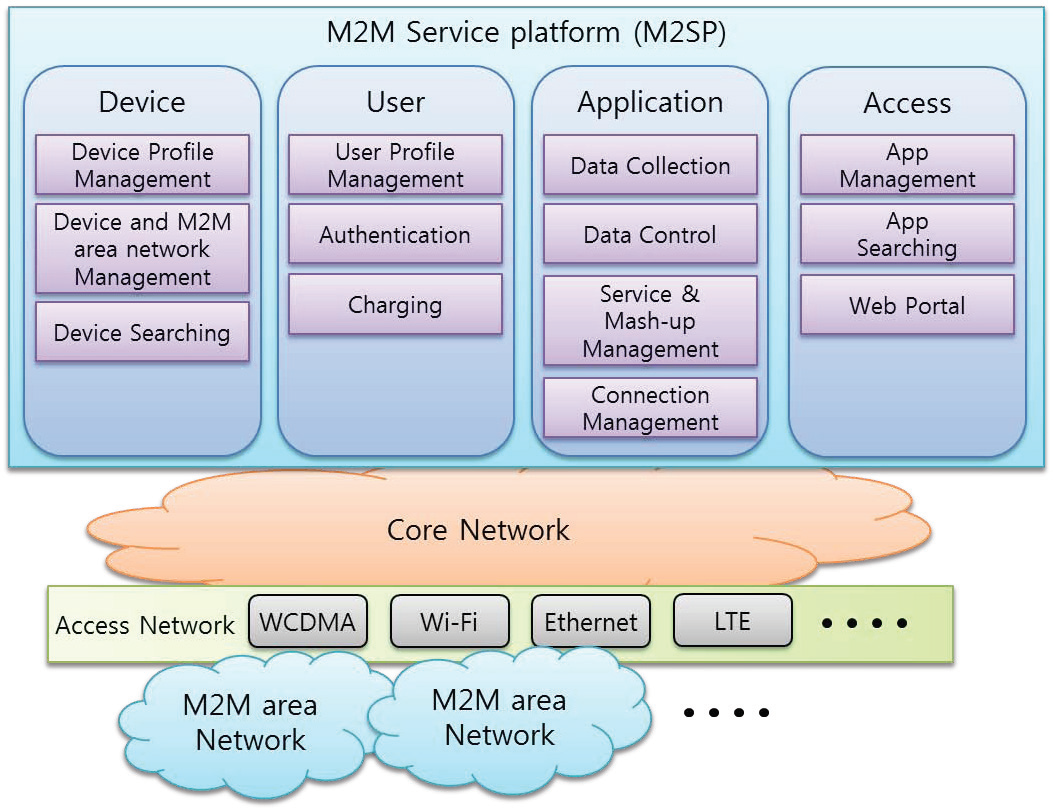
\includegraphics[scale=0.25]{arquitecturaM2SP.png}}
\caption{Arquitectura de la plataforma M2SP}
\label{arqM2SP}
\end{figure}

La plataforma está compuesta por tres tipos de redes: un conjunto de redes M2M, una red de acceso y una red central (core). Las redes M2M son generadas por la interconección de dispositivos bajo sus medios de comunicación; luego, un nodo central recopila información de las redes y se conecta a la red central mediante una red de acceso.\\

En este punto, la red central recibe una enorme cantidad de tráfico con características diferentes, por lo tanto, debe ser capáz de garantizar una buena calidad de servicio a pesar de este tráfico denso y variado.\\

Los usuarios y objetos conectados a la red central pueden acceder a servicios que ofrece la plataforma M2SP, la cual se constituye de 4 entidades.\\

\subsubsection{Plataforma de Dispositivo (M2M Device Platform)}


La plataforma de dispositivos provee acceso a dispositivos registrados a través de la red. Para ello, los dispositivos se registran creando una base de datos con una variedad de información, como tipo de dispositivo, ubicación, descripción, etc.\\
La plataforma tiene la responsabilidad de registrar, modificar y obtener dispositivos. Además, tiene la funcionalidad de manejo de autentificación, monitoreo y control de dispositivos dependiendo de su estado.\\

\subsubsection{Plataforma de Usuario (M2M User Platform)}

La plataforma de usuario tiene la responsabilidad de manejar perfiles de usuario para ofrecer servicios tales como registro, modificación y consulta de información. La plataforma trabaja en conjunto con la plataforma de dispositivos para garantizar accesos de diferentes tipos hacia los dispositivos en la red.\\
De esta forma, los proveedores de servicios y dispositivos tiene privilegios de administrador sobre sus dispositivos y redes de los mismos.\\

\subsubsection{Plataforma de Aplicación (M2M Application Platform)}

La plataforma de aplicación utiliza la información recopilada de los dispositivos para ofrecer diferentes servicios. A partir de los datos disponibles, se proveen diferentes API's para diversos fines.\\

\subsubsection{Plataforma de Acceso (M2M Access Platform)}

La plataforma de acceso provee el servicio de acceso a los demás servicios de la plataforma M2SP a través de aplicaciones o acceso Web. Para aplicaciones en dispositivos inteligentes, la plataforma ofrece la funcionalidad de manejo de aplicaciones que incluye la opción de registro para desarrolladores y mapeo de la aplicación hacia diferentes dispositivos.\\

Adicional a todos estos componentes, la plataforma M2SP opera bajo la arquitectura REST para las interfaces de aplicaciones entre los dispositivos y todos los servicios de la plataforma.\\

De acuerdo a la arquitectura, los autores de \cite{paper1} plantean una plataforma que abarca las principales características que las redes M2M requieren en la actualidad. Mas aún, es una arquitectura diseñada con la posibilidad de interconexión independiente del tipo de red o dispositivo.

\section{Tecnologías y Estandarización}

La implementación de una plataforma de integración como la anteriormente expuesta requiere de ciertas características tecnológicas de los dispositivos para el éxito de la comunicación y operación de los servicios.\\

Este conjunto de características incluyen la identificación y direccionamiento de dispositivos, protocolos de comunicación, manejo de la red, comunicación Pee-to-Peer, y actividades de estandarización.

\subsection{Identificación y direccionamiento}

Dado que la plataforma exige el acceso a los dispositivos por parte de los usuarios, cada uno de ellos debe tener una identificación y dirección única. Para esto, las tecnologías de identificación deben

\section{Caso de estudio: Modelamiento de Redes de Recepción Discontinua (DRX)}

Una característica muy importante de las redes M2M es la eficiencia energética. Esto debido a que la gran mayoría de máquinas que componen las redes son operadas por baterías.

\section{Caso de estudio: Modelamiento de Fuentes de tráfico}
El modelamiento de las fuentes de tráfico es muy importante para dimensionar los requerimientos de la red. Para el caso de las redes M2M, es necesario obtener modelos definidos adecuamente para asi poder conocer los requerimientos a futuro. debido a que se prevé un gran aumento en el número de dispositivos conectados.\\

Para realizar este tipo de modelos existen dos metodologías diferentes. La primera de ellas consiste en modelar simultaneamente el tráfico generado por un gran número de maquinas autónomas por separado. La segunda metodología es la del tráfico agregado, en la cual se acumula el tráfico de todos los dispositivos en un solo flujo.\\
 
Según el articulo \cite{art3}, el modelo de tr\'afico agregado que m\'as se asemeja a las redes M2M es el modelo 3GPP. Sin embargo, se propone un modelo m\'as apropiado utilizando un \emph{Coupled Modulated Markov Poisson Process} (CMPP) porque cada dispositivo se representa como una entidad separada y se tiene en cuenta el acoplamiento debido a la sincronizac\'on del tr\'afico. A continuaci\'on se presenta una descripci\'on de cada uno de los modelos y una comparaci\'on entre ambos.
\subsection{Modelo 3GPP}
Este modelo resulta ser uno de los m\'as utilizados para representar la generaci\'on de tr\'afico en las redes inal\'ambricas y adicionalmente esta relacionado con el funcionamiento de las redes M2M.\\

El modelo 3GPP consiste de dos escenarios llamados Modelo 1 y Modelo 2. El primero de ellos asume que el tr\'afico no est\'a coordinado y la llegada de paquetes tiene una distribuci\'on $f_{T_1}(t)$ uniforme en el intervalo $[0\hspace{4pt}1]$ y el periodo de tiempo $T_1$ es de 60 segundos. El segundo modelo asume que el tr\'afico es sincronizado y la llegada de paquetes tiene una distribuci\'on beta $f_{T_2}(t)=beta(3,4)$ en el intervalo $[0\hspace{4pt}1]$ y el periodo de tiempo $T_2$ es de 10 segundos. Al reescalar ambos intervalos al intervalo $[0\hspace{4pt}T]$ se obtiene la gr\'afica de la distribuci\'on $f_T(t)$ de la Fig.\ref{3GPP1}
\begin{figure}[h]
\centering
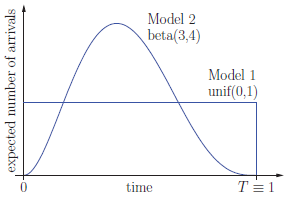
\includegraphics[scale=0.85]{graf1}
\caption{Gr\'afica del n\'umero esperado de llegadas del modelo 3GPP}
\label{3GPP1} 
\end{figure}
El modelo 3GPP se puede ver tambi\'en como un Proceso de Poisson Modulado, en donde se modula la tasa de llegada promedio $\lambda(t)$ en cada intervalo de tiempo $\Delta t$ por una distribuci\'on beta. Esto se observa en la Fig.\ref{3GPP2}.
\begin{figure}[h]
\centering
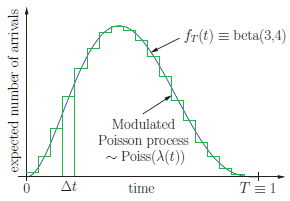
\includegraphics[scale=0.85]{graf2}
\caption{Gr\'afica del n\'umero esperado de llegadas del modelo 3GPP}
\label{3GPP2}
\end{figure} 
Este modelo tiene ciertas limitaciones siguientes limitaciones que impiden cumplir los siguientes los requerimientos de las redes M2M:
\begin{itemize}
\item Se debe asociar una fuente de datos a un lugar fijo 
\item Las r\'afagas de tr\'afico deben provenir de la misma maquina
\item La red influencia los patrones del tr\'afico
\end{itemize}
Para resolver estos problemas, los autores proponen el siguiente modelo.
\subsection{Modelo CMMPP}
En este modelo cada dispositivo es representado coma una entidad independiente, en donde se define la sincronizaci\'on entre todas. Para ello se propone un proceso de fondo que actue como maestro que pueda modular a cada entidad. Cada uno de los dispositivos se representa como un MMPP por separado de la siguiente manera.\\

El caso b\'asico es un MMPP con dos estados, uno de ellos representando operaci\'on normal y el otro operaci\'on bajo alarma, que significa que la tasa de llegada de paquetes es mayor. Para diferenciar la operaci\'on cuando el tr\'afico es coordinado (C) o no coordinado (U) se utilizan las siguientes matrices de transici\'on.
$$\mathbf{P}_U=\left[\begin{array}{cc}
1 & 1\\
0 & 0
\end{array}\right]\hspace{20pt}\mathbf{P}_C=\left[\begin{array}{cc}
0 & 1\\
1 & 0
\end{array}\right]
$$
Para el caso no coordinado se tiene que nunca se va a pasar al estado de alarma y para el caso coordinado disparar una alarma en un intervalo de tiempo y despu\'es regresar a operaci\'on normal. Adicionalmente se tiene que $\lambda_1<\lambda_2=\frac{1}{\Delta t}$\\

Con las Cadenas de Markov acopladas se tiene que hay multiples cadenas que influyen mutuamente en cada una de las matrices de probabilidad de transi\'on $\mathbf{P}_n(t)$. La matriz de la cadena $n$ se multiplica por un factor $\gamma_{n=i|m=j}(t|t-1)$ que depende de los estados pasados $s_m(t-1)$ de la cadena $m$. Para el proposito del modelo desarrollado se tiene una influencia unidireccional del el proceso maestro $\Theta$ hacia cada proceso MMPP.\\

Para encontrar el par\'ametro de influencia del proceso maestro se tiene que este gener\'a muestras $\theta(t)$ en el intervalo $[0\hspace{4pt}1]$ y cada dispositivo tiene un par\'ametro asociado $\delta_n$ constante con lo que se tiene que:
$$\theta_n(t)=\delta_n\cdot\theta(t)$$
A partir dee esto se tiene que la matriz de probabilidad de transici\'on $\mathbf{P}_n(t)$ para el dispositivo $n$ en el tiempo $t$ es:
$$\mathbf{P}_n(t)=\theta_n(t)\cdot \mathbf{P}_C(1-\theta_n(t))\mathbf{P}_U$$
El par\'ametro $\delta_n$ representa la distancia al epicentro y $\theta_n(t)$ es una medida de que tan coordinado es el tr\'afico.

En \cite{art3} se realiza una simulaci\'on del modelo, pero aumentando el n\'umero de estados a 4, en donde los nuevos estados son la fase de \emph{startup} o arranque y el estado de silencio, al cual se pasa si un dispositivo esta en el estado de alarma. La simulaci\'on se realiz\'o para 1000 dispositivos durante 60 segundos y los resultados se muestran a continuaci\'on. Hay que tener en cuenta no se mencionan los cambios en las matrices de transici\'on.

\begin{figure}[h]
\centering
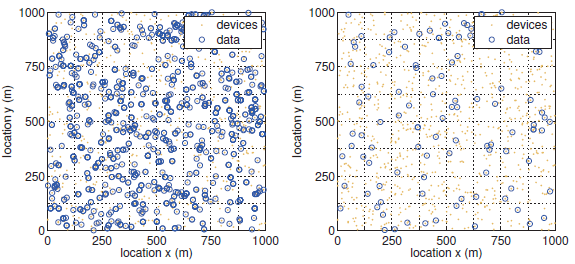
\includegraphics[scale=0.7]{graf3}
\caption{Resultados en el estado de inicio (izquierda) y de operaci\'on regular(derecha)}
\label{CMMPP1}
\end{figure}

En el estado de inicio cada dispositivo intenta transmitir informaci\'on, por lo cual se tiene una gran cantidad de datos. En el estado de operaci\'on normal hay tr\'afico no coordinado distribuido. Posteriormente hay algunos dispositivos en estado de alarma ubicados principalmente en el centro mientras que hay otros que siguen en el estado normal. Por \'ultimo se tiene que en el estado de silencio se distingue que no se generan datos en la zona donde estaba los dispositivos en alarma. De esta manera se observa la transici\'on entre estados de una forma coordinada temporal y espacialmente.

\begin{figure}[h]
\centering
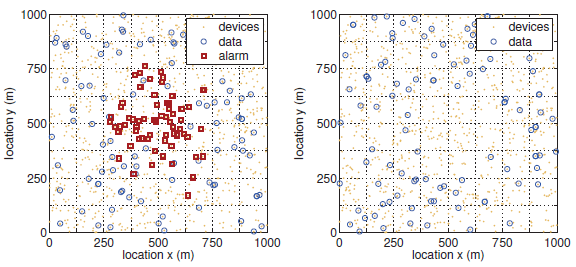
\includegraphics[scale=0.7]{graf4}
\caption{Resultados en el estado alarma (izquierda) y de silencio regular(derecha)}
\label{CMMPP2}
\end{figure}

\subsection{Comparaci\'on entre modelos}
La principal diferencia, como se ha mencionado anteriormente, es que se tiene en cuenta una correlaci\'on espacial y temporal en la generaci\'on del tr\'afico, asi como el modelamiento de cada dispositivo por aparte.

Adicionalmente, en el art\'iculo se lleva a cabo una comparaci\'on en t\'erminos del tiempo requerido para cada simulaci\'on. Para ello se utiliz\'o MatLab para implementar los modelos de 3GPP, 3GPP sequencial (como Proceso de Poisson Modulado) y el CMMPP, teniendo como resultado 0.02 s, 1.1 s y 36 s respectivamente. Adicionalmente se obtuvo una gr\'afica para comparar la duraci\'on de la simulaci\'on a medida que se aumentaba el n\'umero de dispositivos, la cual se muestra en la Fig.\ref{comp}.\\

Se observa que el tiempo de simulaci\'on para ambos modelos 3GPP no aumenta y esto se debe a que son m\'as generales y su complejidad es mucho menor, en la medida que no hay calculos sobre matrices. El modelo de CMMPP tiene un aumento proporcional del tiempo a medida que aumenta los dispositivos, en la medida que hay m\'as cadenas de Markov asociadas pero este resultado es mucho mejor que con otros modelos que tienen en cuenta la coordinaci\'on entre dispositivos independientes.

\begin{figure}[h]
\centering
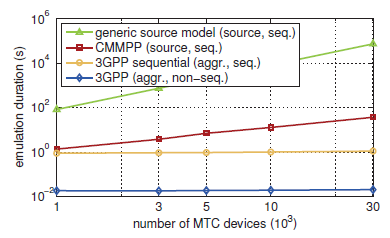
\includegraphics[scale=0.85]{graf5}
\caption{Comparaci\'on del tiempo de simulaci\'on}
\label{comp}
\end{figure}

\section{Conclusiones}



% if have a single appendix:
%\appendix[Proof of the Zonklar Equations]
% or
%\appendix  % for no appendix heading
% do not use \section anymore after \appendix, only \section*
% is possibly needed

% use appendices with more than one appendix
% then use \section to start each appendix
% you must declare a \section before using any
% \subsection or using \label (\appendices by itself
% starts a section numbered zero.)
%

\begin{comment}
\appendices
\section{Proof of the First Zonklar Equation}
Appendix one text goes here.

% you can choose not to have a title for an appendix
% if you want by leaving the argument blank
\section{}
Appendix two text goes here.


% use section* for acknowledgement
\section*{Acknowledgment}


The authors would like to thank...


% Can use something like this to put references on a page
% by themselves when using endfloat and the captionsoff option.
\ifCLASSOPTIONcaptionsoff
  \newpage
\fi



% trigger a \newpage just before the given reference
% number - used to balance the columns on the last page
% adjust value as needed - may need to be readjusted if
% the document is modified later
%\IEEEtriggeratref{8}
% The "triggered" command can be changed if desired:
%\IEEEtriggercmd{\enlargethispage{-5in}}
\end{comment}
% references section

% can use a bibliography generated by BibTeX as a .bbl file
% BibTeX documentation can be easily obtained at:
% http://www.ctan.org/tex-archive/biblio/bibtex/contrib/doc/
% The IEEEtran BibTeX style support page is at:
% http://www.michaelshell.org/tex/ieeetran/bibtex/
%\bibliographystyle{IEEEtran}
% argument is your BibTeX string definitions and bibliography database(s)
%\bibliography{IEEEabrv,../bib/paper}
%
% <OR> manually copy in the resultant .bbl file
% set second argument of \begin to the number of references
% (used to reserve space for the reference number labels box)
\begin{thebibliography}{1}

\bibitem{paper1}
J. ~Kim, J. ~Lee, J. ~Kim and J. ~Yun. ~"M2M Service Platforms: Survey, Issues, and Enabling Technologies", \emph{IEEE Communications Surveys and Tutorials}, Vol. 16, pp. 61-76, 2014.
\bibitem{art3}
M. ~Laner, P. ~Svoboda, N. ~Nikaein and M. ~Rupp. ~'Traffic Models for Machine Type Communications', \emph{Wireless Communication Systems (ISWCS 2013), Proceedings of the Tenth International Symposium on}, pp. 1-5, 2013.
  
\end{thebibliography}

\begin{comment}
% biography section
% 
% If you have an EPS/PDF photo (graphicx package needed) extra braces are
% needed around the contents of the optional argument to biography to prevent
% the LaTeX parser from getting confused when it sees the complicated
% \includegraphics command within an optional argument. (You could create
% your own custom macro containing the \includegraphics command to make things
% simpler here.)
%\begin{IEEEbiography}[{\includegraphics[width=1in,height=1.25in,clip,keepaspectratio]{mshell}}]{Michael Shell}
% or if you just want to reserve a space for a photo:

\begin{IEEEbiography}{Michael Shell}
Biography text here.
\end{IEEEbiography}

% if you will not have a photo at all:
\begin{IEEEbiographynophoto}{John Doe}
Biography text here.
\end{IEEEbiographynophoto}

% insert where needed to balance the two columns on the last page with
% biographies
%\newpage

\begin{IEEEbiographynophoto}{Jane Doe}
Biography text here.
\end{IEEEbiographynophoto}

% You can push biographies down or up by placing
% a \vfill before or after them. The appropriate
% use of \vfill depends on what kind of text is
% on the last page and whether or not the columns
% are being equalized.

%\vfill

% Can be used to pull up biographies so that the bottom of the last one
% is flush with the other column.
%\enlargethispage{-5in}
\end{comment}


% that's all folks
\end{document}


